\documentclass[12pt]{article}

% Opening
\title{Math 3012 Midterm 3}
\author{Akash Narayanan}
\usepackage{amsmath, amsfonts, amssymb, amsthm, enumitem, tikz}
\usepackage{caption, subcaption, float, marginnote, mathtools, mdframed}
\usetikzlibrary{decorations.pathreplacing,decorations.markings}

% Solution environment
\newenvironment{solution}{
\begin{mdframed}
  { {\bfseries Solution}: }}{
\end{mdframed}}

\begin{document}

  \maketitle

  \begin{enumerate}
    \item (20 points) Write the inclusion formula for the number \(d_{n}\) of derangements of \(\{1, 2,\ldots, n\). Then use this formula to calculate \(d_{6}\).

    \begin{solution}
      A derangement is a permutation such that no element is mapped to itself. The formula for the number of derangements is shown below:
      \begin{equation*}
        d_{n} = \sum_{k=0}^{n} (-1)^{k} {n \choose k} (n-k)!
      \end{equation*}
      Letting \(n = 6\), we can calculate that
      \begin{align*}
        d_{6} &= \sum_{k=0}^{6} (-1)^{k} {6 \choose k} (6-k)! \\
              &= {6 \choose 0} 6! - {6 \choose 1} 5! + {6 \choose 2} 4! - {6 \choose 3} 3! + {6 \choose 4} 2! - {6 \choose 5} 1! + {6 \choose 6} 0! \\
              &= 720 - 720 + 360 - 120 + 30 - 6 + 1 \\
              &= 265
      \end{align*}
      That is, there are 265 derangements on a 6-element set.
    \end{solution}

    \pagebreak

    \item (20 points) Write the inclusion-exclusion formula for \(S(n, m)\), the number of surjections from \(\{1, 2, \ldots, n\}\) to \(\{1, 2, \ldots, m\}\). Then use this formula to calculate \(S(6, 4)\).

    \begin{solution}
      The number of surjections from an \(n\)-element set to an \(m\)-element set is
      \begin{equation*}
        S(n, m) = \sum_{k=0}^{m} (-1)^{k} {m \choose k} (m-k)^{n}
      \end{equation*}
      Letting \(n=6, m=4\), we can see that
      \begin{align*}
        S(6, 4) &= \sum_{k=0}^{4} (-1)^{k} {4 \choose k} (4-k)^{6} \\
                &= {4 \choose 0} 4^{6} - {4 \choose 1} 3^{6} + {4 \choose 2} 2^{6} - {4 \choose 3} 1^{6} + {4 \choose 4} 0^{6} \\
                &= 4096 - 2916 + 384 - 4 + 0 \\
                &= 1560
      \end{align*}
      Thus, there are 1560 surjections from a 6-element set to a 4-element set.
    \end{solution}

    \pagebreak

    \item (20 points) Consider the following network flow:

    \begin{figure}[H]
      \begin{center}
        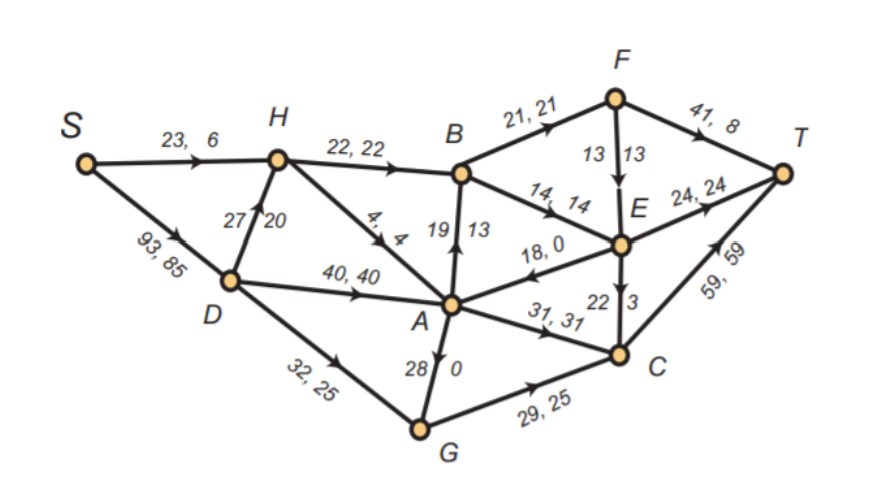
\includegraphics{media/Network Flow.jpg}
      \end{center}
    \end{figure}

    % \begin{figure}[H]
    %   \centering
    %   \begin{tikzpicture}
    %     [scale=1,every node/.style={draw,shape=circle,fill=yellow,inner sep=0,minimum size=6pt},decoration={markings, mark=at position 0.5 with {\arrow[scale=2]{stealth}}}]
    %
    %     \node[label={105:S}] (v1) at (0, 0) {};
    %     \node[label={215:A}] (v2) at (4.25, -1.4) {};
    %     \node[label={90:B}] (v3) at (4.5, -0.2) {};
    %     \node[label={0:C}] (v4) at (6.2, -2.2) {};
    %     \node[label={255:D}] (v5) at (1.5, -1.2) {};
    %     \node[label={85:E}] (v6) at (6.2, -1) {};
    %     \node[label={90:F}] (v7) at (6, 1) {};
    %     \node[label={305:G}] (v8) at (3.75, -3) {};
    %     \node[label={90:H}] (v9) at (2, 0) {};
    %     \node[label={75:T}] (v10) at (8.5, 0) {};
    %
    %     \draw[postaction={decorate}] (v1) -- (v5) node [opacity=0,text opacity=1,scale=0.6,below, pos=0.5, rotate=-45,fill=white] {93, 85};
    %     \draw[postaction={decorate}] (v1) -- (v9) node [opacity=0,text opacity=1,scale=0.6,above, pos=0.5, rotate=0,fill=white] {23, 6};
    %     \draw[postaction={decorate}] (v2) -- (v3) node [opacity=0,text opacity=1,scale=0.6,above, pos=0.5, rotate=0,fill=white] {19, 3};
    %     \draw[postaction={decorate}] (v2) -- (v4) node [opacity=0,text opacity=1,scale=0.6,below, pos=0.5, rotate=-28,fill=white] {31, 31};
    %     \draw[postaction={decorate}] (v5) -- (v2) node [opacity=0,text opacity=1,scale=0.6,above, pos=0.5, rotate=-5,fill=white] {40, 40};
    %     \draw[postaction={decorate}] (v6) -- (v2) node [opacity=0,text opacity=1,scale=0.6,above, pos=0.5, rotate=25,fill=white] {18, 0};
    %     \draw[postaction={decorate}] (v2) -- (v8);
    %     \draw[postaction={decorate}] (v9) -- (v2);
    %     \draw[postaction={decorate}] (v3) -- (v6);
    %     \draw[postaction={decorate}] (v3) -- (v7);
    %     \draw[postaction={decorate}] (v9) -- (v3);
    %     \draw[postaction={decorate}] (v6) -- (v4);
    %     \draw[postaction={decorate}] (v8) -- (v4);
    %     \draw[postaction={decorate}] (v4) -- (v10);
    %     \draw[postaction={decorate}] (v5) -- (v8);
    %     \draw[postaction={decorate}] (v5) -- (v9);
    %     \draw[postaction={decorate}] (v7) -- (v6);
    %     \draw[postaction={decorate}] (v6) -- (v10);
    %     \draw[postaction={decorate}] (v7) -- (v10);
    %   \end{tikzpicture}
    %
    % \end{figure}

    \begin{enumerate}[label=({\alph*})]
      \item (7 points) The value of the current flow is:
      \item (7 points) The capacity of the cut \(\{S, A, D, G, H\} \cup \{B, C, E, F, T\}\) is:
      \item (6 points) Write below the labels that are applied by carrying out the Ford-Fulkerson labeling algorithm.
    \end{enumerate}

    \begin{solution}
      \begin{enumerate}[label=({\alph*})]
        \item The value of the current flow is the flow coming out of the source, which is \(6 + 85 = 91\).
        \item The capacity of a cut is the sum of the capacities over edges going from the set with the source to the set with the sink. The forward edges are AB, AC, GC, and HB. Thus, the capacity of the cut is \(19 + 31 + 29 + 22 = 101\).
        \item We use the Ford-Fulkerson Algorithm and the labelling scheme shown in class.

        \centering
        \begin{tabular}{c c}
          Vertex & Label \\
          S & (*, +, \(\infty\)) \\
          D & (S, +, 8) \\
          H & (S, +, 17) \\
          G & (D, +, 7) \\
          C & (G, +, 4) \\
          E & (C, -, 3) \\
          A & (E, +, 3) \\
          B & (A, +, 3)
        \end{tabular}

        The algorithm halts because all remaining edges from B are either full or have already been accounted for. Thus, the existing flow is maximal. The corresponding cut is \\
        \(\{S, A, B, C, D, E, G\} \cup \{F, H, T\}\). The forward edges are SH, DH, and BF so the cut has capacity \(23 + 27 + 21 = 91\). As expected, this equals the value of the flow.
      \end{enumerate}
    \end{solution}

    \pagebreak

    \item (20 points)
    \begin{enumerate}[label=({\alph*})]
      \item (10 points) Find a particular solution to the advancement operator equation:
      \begin{equation*}
        (A^{2} - 3A + 5) f = 4 \cdot 3^{n}
      \end{equation*}
      \item (10 points) Write the general solution to the homogeneous advancement operator equation:
      \begin{equation}
        [A - (7 - 2i)]^{3} (A - 1)^{4} f = 0
      \end{equation}
    \end{enumerate}

    \begin{solution}
      \begin{enumerate}[label=({\alph*})]
        \item Suppose that a particular solution \(h\) has the form \(h = C \cdot 3^{n}\). Then we have
        \begin{align*}
          (A^{2} - 3A + 5) (C \cdot 3^{n}) &= 4 \cdot 3^{n} \\
          C \cdot 3^{n+2} - 3C \cdot 3^{n+1} + 5C \cdot 3^{n}  &= 4 \cdot 3^{n} \\
          9C \cdot 3^{n} - 9C \cdot 3^{n} + 5C \cdot 3^{n} &= 4 \cdot 3^{n} \\
          5C &= 4 \\
          C = \frac{4}{5}
        \end{align*}
        Thus, we have a particular solution \(h = \frac{4}{5} \cdot 3^{n}\).

        \item We use the theorem describing the general solution to homogeneous recurrence relations. Then the general solution is
        \begin{align*}
          f &= C_{1} \cdot (7 - 2i)^{n} + C_{2} \cdot n (7 - 2i)^{n} + C_{3} \cdot n^{2} (7 - 2i)^{n} \\
          &+ C_{4} + C_{5} \cdot n + C_{6} \cdot n^{2} + C_{7} \cdot n^{3} + C_{8} \cdot n^{4}
        \end{align*}
      \end{enumerate}
    \end{solution}

    \pagebreak

    \item (20 points) Note that \(1800 = 25 \cdot 9 \cdot 8\). Use this information and the inclusion-exclusion formula to determine \(\phi(1800)\), where \(\phi\) is the Euler \(\phi\)-function studied in class.

    \begin{solution}
      We have
      \begin{equation*}
        \phi(n) =  |\{m \in \mathbb{N} : m \leq n, gcd(m,n) = 1\}|
      \end{equation*}
      Suppose \(n\) has the distinct prime factors \(p_{1}, p_{2}, \ldots, p_{k}\). Using the principle of Inclusion-Exclusion, we derived the formula
      \begin{equation*}
        \phi(n) = n\left(1 - \frac{1}{p_{1}}\right) \left(1 - \frac{1}{p_{2}} \right) \cdots \left(1 - \frac{1}{p_{k}} \right)
      \end{equation*}
      We are given that \(1800 = 25 \cdot 9 \cdot 8 = 5^{2} \cdot 3^{2} \cdot 2^{3}\). That is, 1800 has distinct prime factors 2, 3, and 5. Then we use the formula to find that
      \begin{align*}
        \phi(1800) &= 1800 \cdot \frac{1}{2} \cdot \frac{2}{3} \cdot \frac{4}{5} \\
        &= 480
      \end{align*}
    \end{solution}
  \end{enumerate}


\end{document}
